\section{研究与分析}

\subsection{研究目标}

\textbf{\color{red}(描述论文的目标以及成果,目标是解决什么问题/探索新的方向,成果可以是以下几种形式:1发表论文、2申请专利、3获得软件著作权、4开发装置、5开发软件模块或者系统、6构建一个数据集)}

针对XXX领域的不足,研究XXXX方法/开发XXX系统,解决XXX问题或者:探索XXX领域某方面的新思路。研究成果计划发表于XXX会议、申请XXX项发明专利、获得XXX项软件著作权、开发的软件系统将用于XXX、构建的数据集将在学术界公开。

\subsection{研究内容}

\textbf{\color{red}(用一段文字+图说明论文研究内容的设置情况,以及研究内容间的逻辑关系。逻辑关系可以是并列、先后,总分等)}

针对上述问题,本论文的工作分为如下几个方面,如\cref{fig_1}所示。首先研究XXX,在此基础上研究XXX,基于上述研究成果实现XXX。

\begin{figure}[!ht]
	\centering
	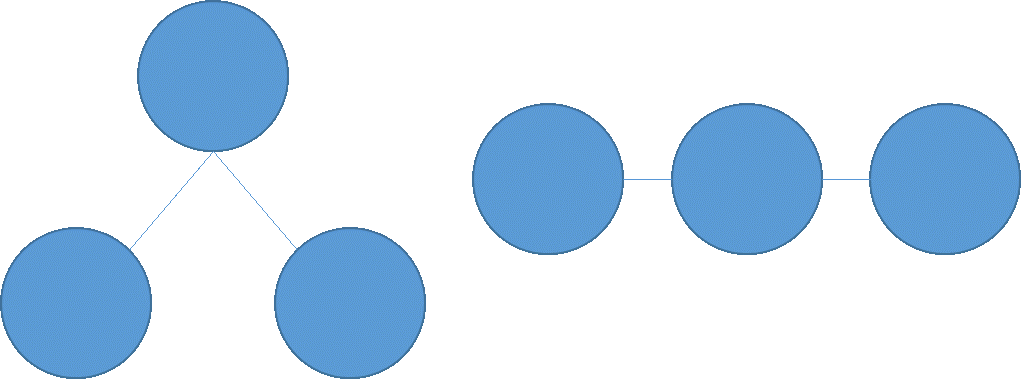
\includegraphics[width=0.4\linewidth]{fig_1.png}
	\caption{研究内容关系示意图}
	\label{fig_1}
\end{figure}

\textbf{\color{red}(下面分别介绍每个研究内容)}

\subsubsection{研究内容一:xxxxxxxxx}

\subsubsection{研究内容二:xxxxxxxxx}

\subsubsection{研究内容三:xxxxxxxxx}


\subsection{拟解决的实际工程问题}


\subsection{拟采取的研究方法、技术路线}

\textbf{\color{red}(下面通过图文的形式说明论文技术方案)}

\subsubsection{XXXXX方法技术路线}

本文使用XXX方法技术路线,如\cref{fig_2}所示。

\begin{figure}[ht]
	\centering
	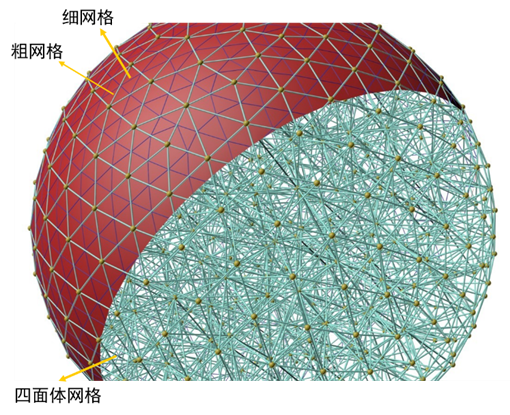
\includegraphics[width=0.6\linewidth]{fig_2.png}
	\caption{本论文拟构建的物理仿真模型示意图}
	\label{fig_2}
\end{figure}

\subsubsection{XXXXX方法技术路线}

\subsubsection{XXXXX方法技术路线}

\subsection{预期创新点}
\textbf{\color{red}(描述论文工作的创新性,与现有研究和工程方案的区别,侧重于理论方法研究的论文可以写方法思路的创新性,侧重于工程实践的论文,可以写系统方案、解决问题的新思路)}

论文将引入XXX思路、改进XXX方法、探索XXX理论,从而提高XXX准确率,实现XXX效果、解决XXX问题。

\clearpage
